\documentclass{article}
\usepackage[utf8]{inputenc}
\usepackage[margin=1.2in]{geometry}
\usepackage{graphicx}
\usepackage{xcolor}
\usepackage{listings}
\usepackage{float}
\usepackage{subcaption}
\lstset{
  language=python,
  columns=fullflexible,
  frame=single,
  breaklines=true,
  moredelim=**[is][\color{red}]{@}{@}
}

\title{Machine Learning}
\author{Martin Guyard et Guillaume Brizolier}
\date{TP2 : Renewable Energy Prediction}

\begin{document}

\maketitle

\section{Preprocessing des données}
\subsection{Problèmes éventuels dans les données}
\begin{enumerate}
    \item Redondance : cela peut éventuellement ralentir les calculs mais ce n'est pas un problème en soi.
    \item Normalisation : Il faut toujours normaliser pour des problèmes informatiques ! On divise chaque colonne par la valeur max et on soustrait la moyenne pour centrer les données.
    \item Indépendance : fortement lié à la redondance. Dans notre cas, ce n'est pas un problème.
    \item Format : Utilisation de one-hot vector pour convertir les chaînes ASCII en un nombre de colonnes égales au nombre de villes. Il s'agit d'un vecteur où toutes les valeurs sont nulles sauf 1 à 0 qui correspond à l'indicateur de catégorie.
    
     \begin{center}
    \begin{tabular}{c|c|c|c|c|c}
        0 & 0 & 0 & 1 & 0 & 0  \\
    \end{tabular}
    \end{center}
    On utilise la même technique pour la date avec cette fois-ci 3 one-hot vectors : un de 12 cases pour les mois, un de 31 pour les jours, et un de 24 pour les heures.
    \item Trous : Si on a des trous, on peut soit faire des moyennes pondérées en fonction de points suivants et précédents, ou tout simplement remplacée par la moyenne (nulle ici car nous avons normalisé les données).\\
    \end{enumerate}
    \subsection{Input}
    [9, Nbcol, 1] : on a un seul neurone qui est un réel.
    Output : [batch, 1]
    Dans notre couche finale, on fait une combinaison linéaire qui sort un nombre sans mettre de fonction d'activation, puisqu'on veut des valeurs dans R.\\
    Au milieu : on met une couche dense fully connected, et ça marche. Les fonctions d'activation au sein du réseau sont celles qu'on veut, mais par contre à celle de la fin on n'en met pas.
    \section{Prévision}
    target : une ligne!\\ on peut utiliser une fenêtre de 4 lignes.
    Input : [9 : nb de lignes, 4 : nb de dimensions tempo que je veux, NbCol : nbre de features] : b(batch), t(time), c(colonnes)\\
    Je ne peux prédire qu'une valeur ! (pas toute la ligne). Du coup la sortie ne change pas.
    \section{Modèles utilisés}
    \subsection{Modèle régressif}
    Ce problème de prédiction pouvant s'assimiler à un problème de régression, nous avons choisi d'utiliser un SVR (\textit{Support Vector Regression}), importé depuis le module \textit{sklearn}.
    \begin{lstlisting}[frame=single]
        from sklearn.svm import SVR

        def model_no_ann(name, data, idx, target):
    """ Train a model on train + valid data set
    # Argument
        :param name: str, name
        :param data: numpy array, data
        :param idx: dict, data sets indexes
        :param target: int, position of target
    """
        fn = join(model_path, name)
        dt = np.concatenate((data[idx['train'], :target], data[idx['train'], target + 1:]), axis=-1)
        dv = np.concatenate((data[idx['valid'], :target], data[idx['valid'], target + 1:]), axis=-1)
        dtv = np.concatenate((dt, dv))
        ltv = np.concatenate((data[idx['train'], target], data[idx['valid'], target]))
        @model = SVR(epsilon=0.001)
        model.fit(dtv, ltv)@
        '''
        === Put some code here ===
        '''
        with open(fn, 'wb') as f:
            pidump(model, f)
        dtest = np.concatenate((data[idx['test'], :target], data[idx['test'], target + 1:]), axis=-1)
        graph_comparison([model.predict(dtest)], data, idx, target, 1, 0, t_idx='test', step=200)
    \end{lstlisting}
    Ici, le kernel utilisé est 'rbf' (paramètre par défaut) car les données ne sont pas linéairement séparables. On garde tous les autres paramètres à leur valeur par défaut, mis à part epsilon qu'on choisit à 0.001 pour un maximum de précision. Comme le montre les courbes de prédictions suivantes, le modèle prédit parfaitement les données de test :
    \begin{figure}
        \centering
        \begin{subfigure}{.5\textwidth}
          \centering
          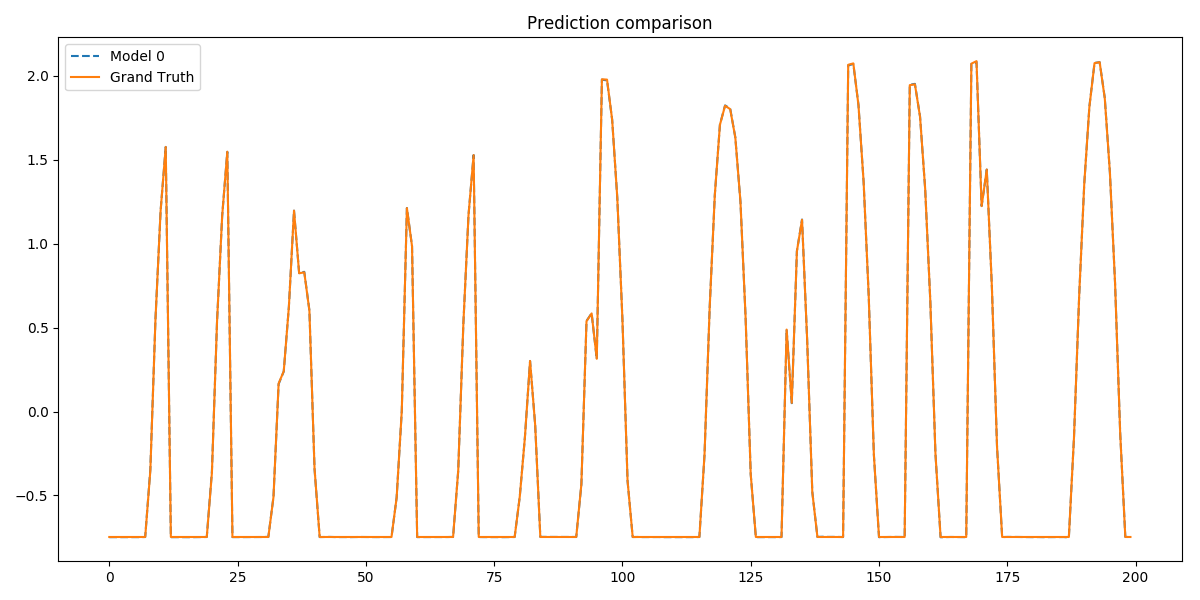
\includegraphics[scale=0.25]{comparison_test_0.png}
          \caption{Comparaison 1}
          \label{fig:sub1}
        \end{subfigure}%
        \begin{subfigure}{.5\textwidth}
          \centering
          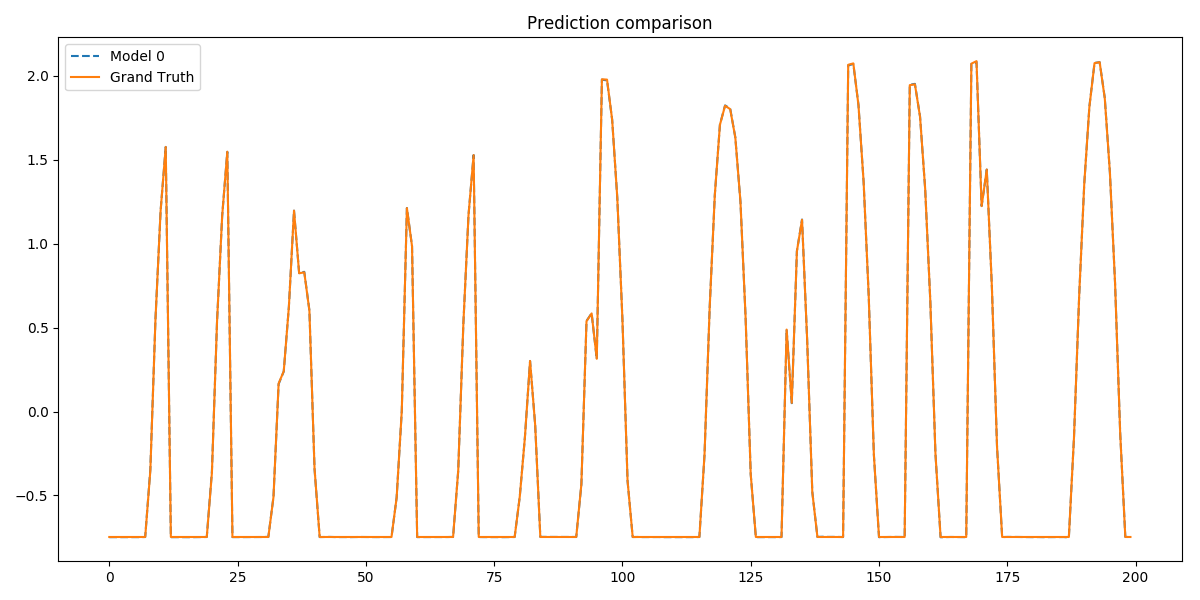
\includegraphics[scale=0.25]{comparison_test_0.png}
          \caption{Comparaison 2}
          \label{fig:sub2}
        \end{subfigure}
        \caption{Données de test (orange solide) vs données prédites par le modèle (bleu pointillé)}
        \label{fig:test}
    \end{figure}
    Nous obtenons donc des performances très satisfaisantes pour ce modèle.
    \subsection{Modèle Réseau de Neurones}
    Nous avons choisi une architecture relativement simple pour notre réseau de neurones. Nous avons choisi de faire un ANN fully-connected, avec 3 couches dense : la première avec 500 neurones, la deuxième avec 100, la troisième avec 10, complétée par une dernière couche d'une seule neurone sans fonction d'activation pour avoir le résultat final de la prédiction.\\\\Le code correspondant, écrit avec l'API fonctionnelle de Keras, est le suivant :\\\\\\\\\\\\
    \begin{lstlisting}[frame=single]
        def create_model(w, c):
        """ Create a keras model
        # Arguments
            :param w: int, time dimension
            :param c: int, channel dimension
        # Returns
            :return: keras model
        """
        l_in = Input(shape=(w, c,))  
        
        l_hidden_0 = Dense(500, activation='relu')(l_in)
        l_hidden_1 = Dense(100, activation='relu')(l_hidden_0)
        l_hidden_2 = Dense(10, activation='relu')(l_hidden_1)
        l_hidden_3 = Dense(1)(l_hidden_2)
        l_out = Flatten()(l_hidden_3)

        return Model(l_in, l_out)
    \end{lstlisting}

    On remarque qu'on utilise un layer Flatten au début. Cela est en fait dû aux différences de dimensions de l'input du modèle, qui doit correspondre aux dimensions données par les fonctions de générations de données, à savoir [batch, fenêtre, canaux], tandis que l'output lui correspond simplement à la dimension du batch.

    Les résultats pour ce modèle sont un peu moins convaincants, pour une raison que nous ne sommes pas arrivés à déterminer le modèle ne semble pas converger vers une valeur de loss satisfaisante.
    Voici les résultats que nous obtenons :\\
    \begin{figure}[H]
        \centering
        \begin{subfigure}[t]{0.49\textwidth}
            \raisebox{-\height}{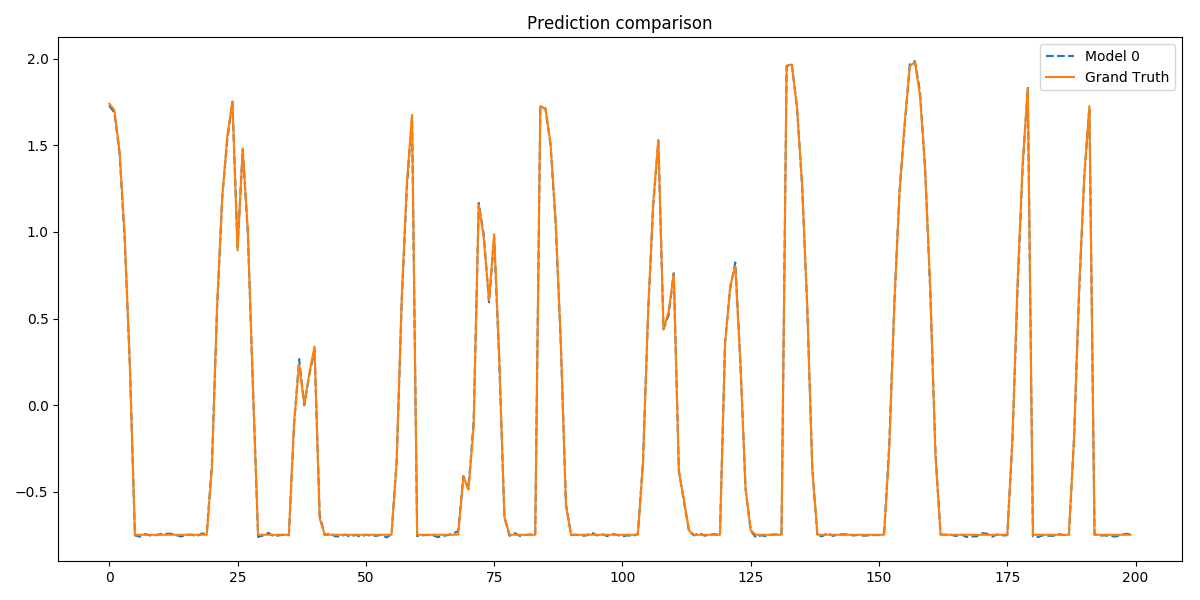
\includegraphics[width=\textwidth]{comparison_valid_0.png}}
            \caption{caption of first image}
        \end{subfigure}
        \hfill
        \begin{subfigure}[t]{0.49\textwidth}
            \raisebox{-\height}{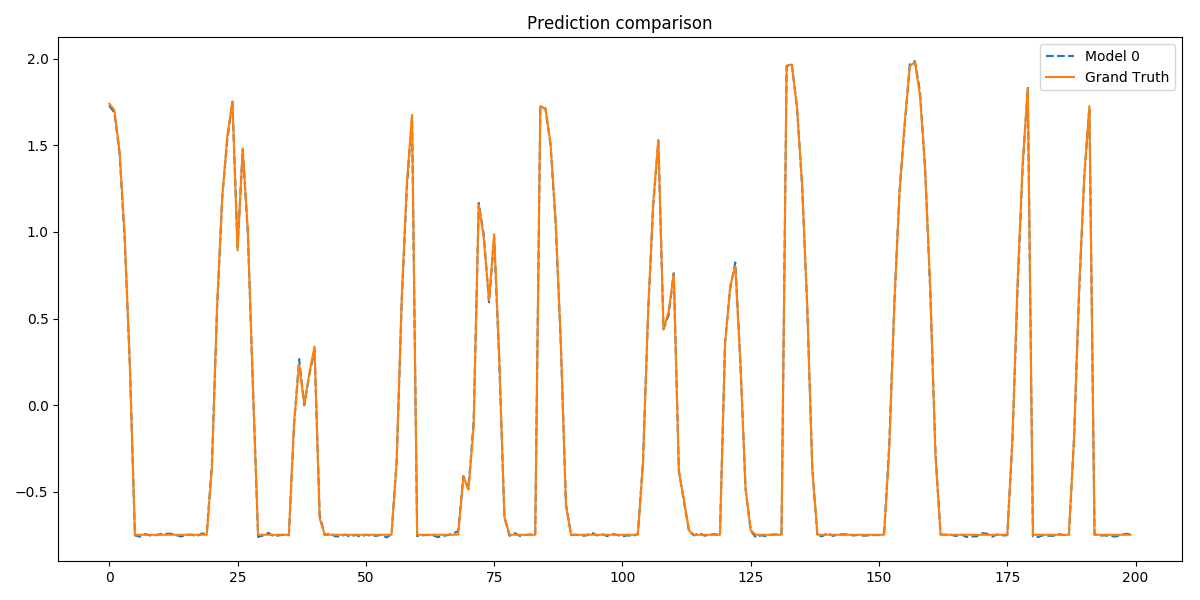
\includegraphics[width=\textwidth]{comparison_valid_0.png}}
        \caption{caption of second image\\second line}
    \end{subfigure}
        \caption{Données de validation (orange solide) vs données prédites par le modèle (bleu pointillé)}
        \label{fig:test}
    \end{figure}
    \begin{figure}[H]
        \centering
        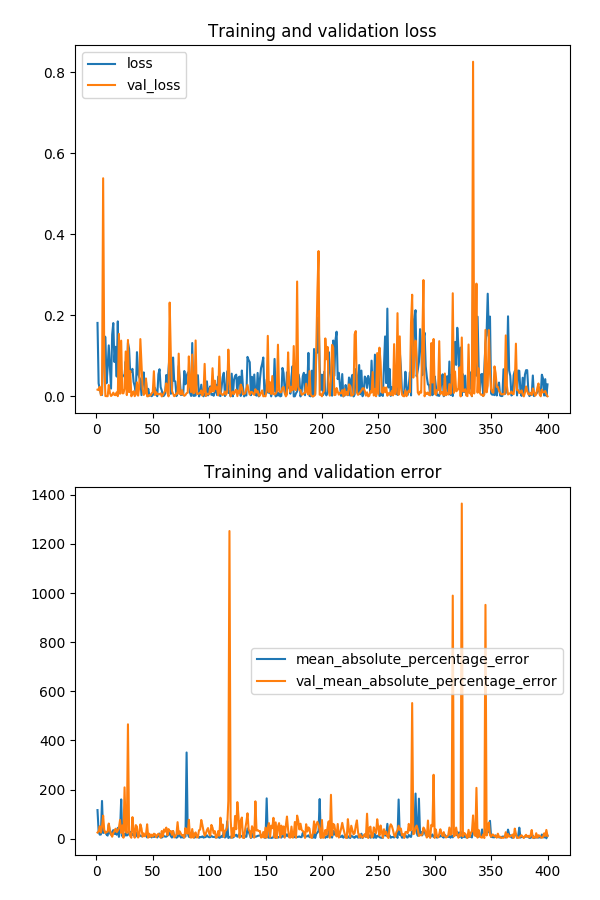
\includegraphics[scale=0.5]{results.png}
        \caption{Loss et Mean Squared Error en fonction du nombre de batch}
        \label{fig:schema}
    \end{figure}
    
\end{document}
